% Options for packages loaded elsewhere
\PassOptionsToPackage{unicode}{hyperref}
\PassOptionsToPackage{hyphens}{url}
\documentclass[
  10pt,
]{article}
\usepackage{xcolor}
\usepackage[margin=0.8in]{geometry}
\usepackage{amsmath,amssymb}
\setcounter{secnumdepth}{-\maxdimen} % remove section numbering
\usepackage{iftex}
\ifPDFTeX
  \usepackage[T1]{fontenc}
  \usepackage[utf8]{inputenc}
  \usepackage{textcomp} % provide euro and other symbols
\else % if luatex or xetex
  \usepackage{unicode-math} % this also loads fontspec
  \defaultfontfeatures{Scale=MatchLowercase}
  \defaultfontfeatures[\rmfamily]{Ligatures=TeX,Scale=1}
\fi
\usepackage{lmodern}
\ifPDFTeX\else
  % xetex/luatex font selection
\fi
% Use upquote if available, for straight quotes in verbatim environments
\IfFileExists{upquote.sty}{\usepackage{upquote}}{}
\IfFileExists{microtype.sty}{% use microtype if available
  \usepackage[]{microtype}
  \UseMicrotypeSet[protrusion]{basicmath} % disable protrusion for tt fonts
}{}
\makeatletter
\@ifundefined{KOMAClassName}{% if non-KOMA class
  \IfFileExists{parskip.sty}{%
    \usepackage{parskip}
  }{% else
    \setlength{\parindent}{0pt}
    \setlength{\parskip}{6pt plus 2pt minus 1pt}}
}{% if KOMA class
  \KOMAoptions{parskip=half}}
\makeatother
\usepackage{longtable,booktabs,array}
\newcounter{none} % for unnumbered tables
\usepackage{calc} % for calculating minipage widths
% Correct order of tables after \paragraph or \subparagraph
\usepackage{etoolbox}
\makeatletter
\patchcmd\longtable{\par}{\if@noskipsec\mbox{}\fi\par}{}{}
\makeatother
% Allow footnotes in longtable head/foot
\IfFileExists{footnotehyper.sty}{\usepackage{footnotehyper}}{\usepackage{footnote}}
\makesavenoteenv{longtable}
\usepackage{graphicx}
\makeatletter
\newsavebox\pandoc@box
\newcommand*\pandocbounded[1]{% scales image to fit in text height/width
  \sbox\pandoc@box{#1}%
  \Gscale@div\@tempa{\textheight}{\dimexpr\ht\pandoc@box+\dp\pandoc@box\relax}%
  \Gscale@div\@tempb{\linewidth}{\wd\pandoc@box}%
  \ifdim\@tempb\p@<\@tempa\p@\let\@tempa\@tempb\fi% select the smaller of both
  \ifdim\@tempa\p@<\p@\scalebox{\@tempa}{\usebox\pandoc@box}%
  \else\usebox{\pandoc@box}%
  \fi%
}
% Set default figure placement to htbp
\def\fps@figure{htbp}
\makeatother
\setlength{\emergencystretch}{3em} % prevent overfull lines
\providecommand{\tightlist}{%
  \setlength{\itemsep}{0pt}\setlength{\parskip}{0pt}}
\usepackage{bookmark}
\IfFileExists{xurl.sty}{\usepackage{xurl}}{} % add URL line breaks if available
\urlstyle{same}
\hypersetup{
  pdftitle={HarmonyXR GazePose-Context: Multimodal Context Inference for Adaptive XR Training},
  pdfauthor={Lavanya D.},
  hidelinks,
  pdfcreator={LaTeX via pandoc}}

\title{HarmonyXR GazePose-Context: Multimodal Context Inference for
Adaptive XR Training}
\author{Lavanya D.}
\date{May 14, 2026}

\begin{document}
\maketitle

\section{Abstract}\label{abstract}

Adaptive extended reality (XR) systems require more than object
interaction; they require an ability to understand whether a user is
focused, distracted, transitioning between steps, or inactive. This
paper presents HarmonyXR GazePose-Context, a Unity and Meta Quest
proof-of-concept that infers user context during a guided XR sorting
task using runtime signals available in the current headset-facing
implementation. The system uses a three-layer architecture: sensor
abstraction, context inference, and XR app shell adaptation. Runtime
evidence was collected from a Quest headset run using Unity console
logs, filtered QA evidence, processed CSV tables, and a headset video.
The evidence run produced 169 QA metric samples and captured all four
target context states: Engaged, Distracted, Transitioning, and Idle. The
results support the feasibility of a lightweight, interpretable adaptive
XR prototype that uses multimodal context signals to drive user-facing
guidance. The work is positioned as headset-running prototype evidence;
a formal participant study remains future Phase 4 work.

\textbf{Keywords:} extended reality, adaptive XR, context inference,
gaze, hand tracking, posture, multimodal interaction, Unity, Meta Quest

\section{1. Introduction}\label{introduction}

XR training systems increasingly need to support users who shift between
focused task execution, attention loss, transitional movement, and
inactivity. Traditional XR applications often respond only to explicit
controller input or predefined task events. This limits the system's
ability to provide timely help when the user is distracted, paused, or
moving between task steps.

HarmonyXR GazePose-Context addresses this problem through a lightweight
multimodal context inference prototype. The system observes runtime
signals from the XR scene, combines them into a shared signal frame,
infers one of four user context states, and exposes adaptive support in
the XR app shell. The user task is intentionally simple: sort virtual
objects into matching targets. This keeps the research focus on context
inference and adaptive response rather than game complexity.

The main contribution of this work is not a new game mechanic or a full
user study. It is a working headset-facing proof-of-concept that
demonstrates how multimodal XR runtime signals can support context-aware
behavior during a controlled training task.

The contributions are:

\begin{enumerate}
\def\labelenumi{\arabic{enumi}.}
\tightlist
\item
  A three-layer implementation structure for adaptive XR context
  inference.
\item
  A headset-facing prototype that captures gaze/AOI evidence, spatial
  context, hand interaction, pinch state, and gaze timing features
  available in the current runtime.
\item
  A four-state context model covering Engaged, Distracted,
  Transitioning, and Idle behavior.
\item
  A user-facing adaptive XR shell that communicates context state and
  task guidance.
\item
  A runtime evidence package containing a headset video, console logs,
  filtered state evidence, and processed tables.
\end{enumerate}

\section{2. Related Work}\label{related-work}

The paper is positioned across five areas of XR research: gaze and
attention in immersive environments, multimodal attention detection,
body and hand tracking, multimodal XR interaction, and context-aware XR
adaptation.

\subsection{2.1 Gaze Tracking and Attention in
VR}\label{gaze-tracking-and-attention-in-vr}

Eye tracking is widely used in VR to estimate attention, object focus,
dwell behavior, and gaze-based interaction. Moreno-Arjonilla et
al.~survey VR eye-tracking hardware, calibration, gaze estimation
methods, datasets, and application areas, showing that gaze is a
foundational signal for immersive interaction and attention analysis
{[}1{]}. However, the survey also makes clear that gaze-centric systems
do not by themselves capture full user context, because they typically
do not integrate body pose, task events, or broader behavioral signals.

Pastel et al.~compare gaze accuracy and precision between real-world and
VR conditions {[}2{]}. Their results show that gaze can be useful in
controlled static tasks, but accuracy and precision become more
difficult under dynamic conditions. This supports the design decision in
HarmonyXR GazePose-Context to avoid relying on gaze/AOI evidence alone
and instead combine it with hand, posture, spatial, and task-related
signals.

\subsection{2.2 Multimodal Attention and XR
Interaction}\label{multimodal-attention-and-xr-interaction}

Long et al.~demonstrate that multimodal physiological sensing can
improve classification of internal and external attention in VR by
combining EEG and eye-tracking features {[}3{]}. This supports the
broader claim that multimodal sensing can improve attention-state
inference. At the same time, their approach depends on specialized EEG
hardware and uses time windows that are larger than the lightweight
runtime loop used in the current prototype. HarmonyXR therefore focuses
on behavioral and interaction signals that can be collected inside an XR
application without adding brain-computer-interface hardware.

Rakkolainen et al.~provide a scoping review of multimodal interaction
technologies in extended reality, covering gaze, gestures, speech,
haptics, physiological sensing, and other modalities {[}4{]}. Kim et
al.~later analyze the chronological shift from controller-based
interaction toward hand, gaze, wrist, voice, and multimodal input across
XR device generations {[}5{]}. Together, these reviews show that XR
interaction is moving toward multimodal input, but they also highlight a
gap between collecting multiple input channels and using those channels
for real-time behavioral context inference.

\subsection{2.3 Body, Head, and Hand
Tracking}\label{body-head-and-hand-tracking}

Body and posture signals provide useful evidence about user behavior
beyond visual attention. Bustamante et al.~show that skeleton-based
posture recognition can classify standing, sitting, and lying using
lightweight geometric heuristics {[}6{]}. Neidhardt et al.~show that
head-mounted XR tracking can provide useful evidence about body movement
during VR-based musculoskeletal training {[}7{]}. These works support
the use of posture and movement signals, but they focus mainly on
physical-state estimation rather than combining pose with gaze/AOI and
task-state evidence for adaptive XR behavior.

Hand interaction is another important behavioral signal in XR because it
indicates whether the user is actively manipulating or approaching task
objects. Lei et al.~propose a sensor-fusion approach for precise hand
tracking in VR using multiple sensing sources and temporal modeling
{[}8{]}. Their work focuses on improving hand-tracking accuracy, while
HarmonyXR uses hand and pinch evidence as part of a higher-level context
inference model.

\subsection{2.4 Gaze-Based Feedback and Context-Aware
Adaptation}\label{gaze-based-feedback-and-context-aware-adaptation}

Selaskowski et al.~present gaze-based attention refocusing training in
VR for adults with ADHD {[}9{]}. Their system uses gaze behavior to
trigger feedback when attention shifts away from a continuous
performance task, while also collecting EEG, head movement, and
performance measures for analysis. This work is relevant because it
shows how gaze behavior can drive real-time feedback, but its online
decision logic remains primarily gaze-based rather than a fused
multimodal context model.

Davari and Bowman propose a design space for context-aware XR interfaces
and evaluate an adaptive placement strategy for XR content {[}10{]}.
Their work demonstrates the importance of context-aware adaptation for
usability and cognitive load, but the context reasoning is primarily
about interface placement and environmental relevance. Ramiotis and
Mania propose CONTEXT-GAD, a context-aware adaptive dwell model that
combines gaze behavior, head rotation, interaction frequency, and scene
context to adapt gaze dwell thresholds {[}11{]}. This shows that recent
XR research is moving from gaze-only interaction toward context-aware
adaptation, but the adaptation remains centered on gaze selection rather
than general user-context inference.

\subsection{2.5 Research Gap}\label{research-gap}

Existing XR research shows strong progress in gaze tracking, multimodal
sensing, body/posture recognition, hand tracking, and context-aware
interface adaptation. However, these strands are often treated
separately: gaze systems focus on attention or selection, posture
systems focus on body-state classification, hand-tracking systems focus
on tracking accuracy, and context-aware XR systems often adapt placement
or feedback based on narrow context definitions. HarmonyXR
GazePose-Context addresses this gap at prototype level by combining
runtime gaze/AOI evidence, hand interaction, posture or spatial context,
and task-related signals into an interpretable four-state context model
that drives adaptive XR support.

\section{3. Research Problem and
Scope}\label{research-problem-and-scope}

The research problem is: how can an XR system infer user context from
lightweight runtime signals and use that inference to support adaptive
behavior during a training task?

The current paper focuses on prototype implementation and evidence-based
validation. It does not claim a completed participant study or
statistical comparison. Phase 4 user study work is treated as future
work.

The current scope includes:

\begin{itemize}
\tightlist
\item
  Unity and Meta Quest headset execution.
\item
  TrainingSimulation sorting task.
\item
  Four context states: Engaged, Distracted, Transitioning, Idle.
\item
  Runtime QA metrics and context-state evidence.
\item
  Adaptive support and completion feedback inside the XR experience.
\end{itemize}

The current scope excludes:

\begin{itemize}
\tightlist
\item
  New gameplay systems.
\item
  Phone/mobile support.
\item
  Formal user study statistics.
\item
  NASA-TLX results.
\item
  Baseline-versus-adaptive participant comparison.
\end{itemize}

\section{4. System Overview}\label{system-overview}

The implementation follows the three-layer structure defined in the
implementation guide and WBS: Sensor Abstraction, Context Engine, and XR
App Shell. Figure 1 summarizes the runtime pipeline.

\begin{figure}
\centering
\pandocbounded{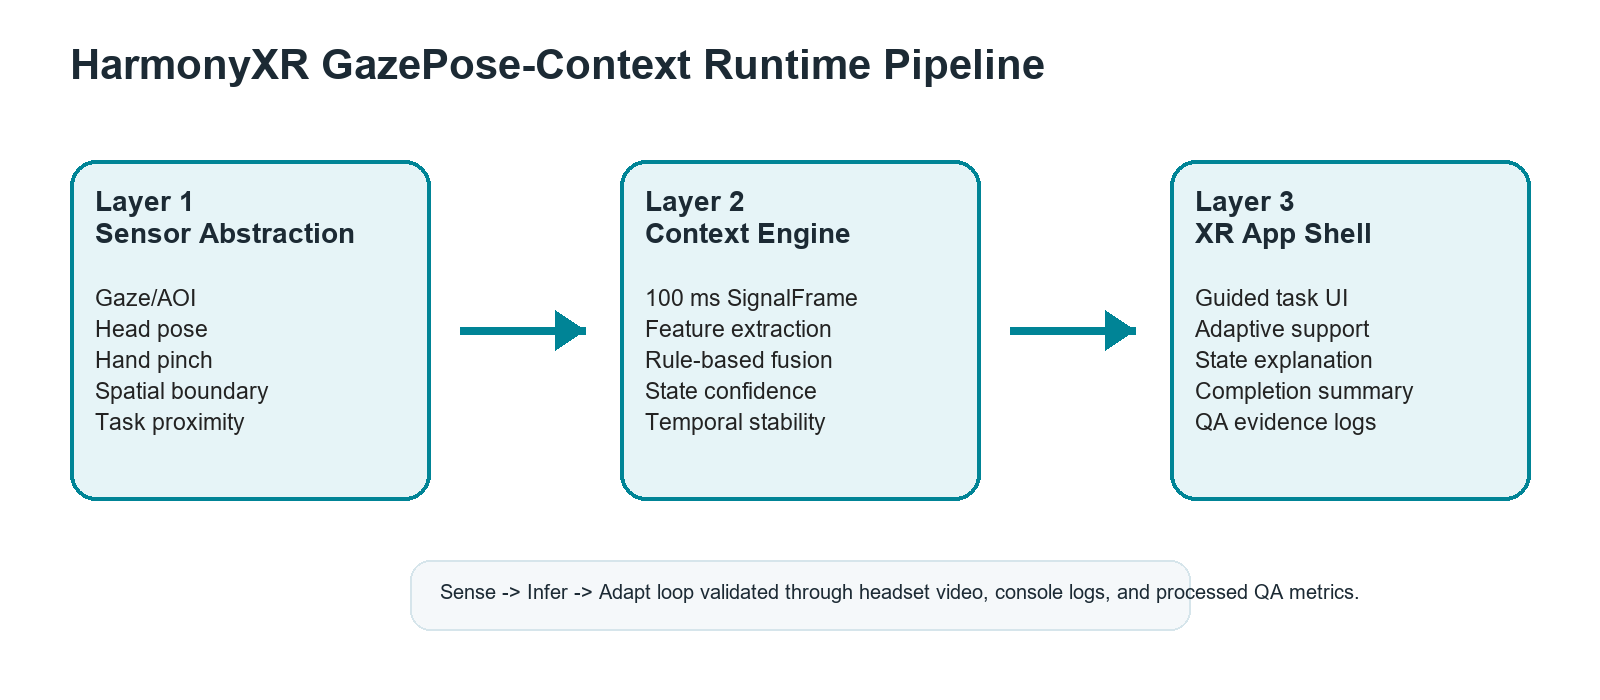
\includegraphics[keepaspectratio,alt={HarmonyXR GazePose-Context runtime pipeline.}]{figures/figure1_runtime_pipeline.png}}
\caption{HarmonyXR GazePose-Context runtime pipeline.}
\end{figure}

\subsection{4.1 Layer 1: Sensor
Abstraction}\label{layer-1-sensor-abstraction}

The sensor abstraction layer converts headset and scene signals into
runtime fields. Relevant fields include AOI, posture or spatial posture
context, boundary mode, fixation duration, dwell ratio, saccade rate,
body activity, hand interaction count, pinch state, and distance to task
object. These are emitted through QA metrics and logged for validation.

\subsection{4.2 Layer 2: Context Engine}\label{layer-2-context-engine}

The context engine consumes the synchronized signal frame and infers a
context state. The current implementation uses interpretable rule-based
logic and confidence values rather than a black-box model. This design
keeps the proof-of-concept explainable for research and stakeholder
review.

\subsection{4.3 Layer 3: XR App Shell}\label{layer-3-xr-app-shell}

The XR app shell translates inferred state into visible user support. It
includes onboarding, task guidance, context-aware feedback, adaptive
support actions, QA/evidence logging, and end-of-session completion
messaging.

\section{5. Prototype Implementation}\label{prototype-implementation}

The prototype is implemented in Unity 2022.3.62f1 with OpenXR 1.14.3 and
Meta XR SDK 201.0.0. The app targets Meta Quest headset execution. The
primary scene is TrainingSimulation, where the user sorts a cube,
cylinder, and sphere into corresponding pads or receptacles.

The main implementation components are:

\begin{itemize}
\tightlist
\item
  \textbf{SignalSynchroniser:} emits runtime signal frames on a 100 ms
  cadence.
\item
  \textbf{ContextDebugTester / context pipeline:} evaluates context
  state and confidence.
\item
  \textbf{TrainingSimulationUserGuide:} presents onboarding, task
  guidance, incorrect-object messaging, and completion summary.
\item
  \textbf{AdaptationManager:} maps inferred context states to adaptive
  XR support and QA metric console logging.
\item
  \textbf{ContextLogger:} records context output for analysis.
\end{itemize}

The proof-of-concept intentionally stays within a narrow research scope.
It does not add unrelated gameplay or study-management systems. The goal
is to show that adaptive XR behavior can be driven by inferred context
signals during a simple task.

\section{6. Context State Model}\label{context-state-model}

The system infers four context states.

\textbf{Engaged} indicates that the user is focused on task-relevant
content or interacting with the current task. It represents active task
participation.

\textbf{Distracted} indicates that attention has shifted away from the
task or that task-directed activity is reduced. It supports refocus
guidance.

\textbf{Transitioning} indicates movement between task steps, targets,
or interaction states. It supports soft guidance while the user changes
focus.

\textbf{Idle} indicates low activity, little interaction, or a pause
state. It supports rest, recentering, or continuation options.

These states are used as runtime categories for adaptive behavior and
evidence reporting. They are not clinical or psychological diagnoses.

\section{7. Evidence Collection
Method}\label{evidence-collection-method}

Evidence was collected through a combined headset evidence run on May
14, 2026. ADB logcat captured Unity runtime console output while the
application ran in the Quest headset. The collected artifacts were
organized under \texttt{Research\_Evidence}.

Primary evidence files include:

\begin{itemize}
\tightlist
\item
  \texttt{03\_Context\_State\_Coverage/20260514\_run01\_full-evidence.mp4}
\item
  \texttt{05\_Stability\_Latency/20260514\_run01\_console-evidence.txt}
\item
  \texttt{05\_Stability\_Latency/20260514\_run01\_filtered-evidence.txt}
\item
  \texttt{07\_Processed\_Tables\_Charts/qa\_metrics\_extract.csv}
\item
  \texttt{07\_Processed\_Tables\_Charts/state\_coverage\_table.csv}
\item
  \texttt{07\_Processed\_Tables\_Charts/adaptation\_event\_table.csv}
\item
  \texttt{07\_Processed\_Tables\_Charts/stability\_latency\_table.csv}
\end{itemize}

The evidence run produced 169 QA metric samples. Each QA metric line
contained state, confidence, boundary, AOI, posture/spatial context,
fixation, dwell, saccade, body activity, hand interaction count, pinch
state, and distance to task object.

\section{8. Results}\label{results}

\subsection{8.1 Context State Coverage}\label{context-state-coverage}

All four required context states appeared in the headset evidence run.

{\def\LTcaptype{none} % do not increment counter
\begin{longtable}[]{@{}lrlll@{}}
\toprule\noalign{}
State & Samples & First timestamp & Last timestamp & Found \\
\midrule\noalign{}
\endhead
\bottomrule\noalign{}
\endlastfoot
Engaged & 15 & 05-14 16:19:18.956 & 05-14 16:21:33.401 & Yes \\
Distracted & 30 & 05-14 16:16:46.104 & 05-14 16:21:55.453 & Yes \\
Transitioning & 100 & 05-14 16:19:28.044 & 05-14 16:21:48.434 & Yes \\
Idle & 24 & 05-14 16:16:49.126 & 05-14 16:22:02.470 & Yes \\
\end{longtable}
}

\begin{figure}
\centering
\pandocbounded{
\includegraphics[keepaspectratio,alt={Context state sample counts observed in the headset evidence run.}]{figures/figure2_state_coverage.png}}
\caption{Context state sample counts observed in the headset evidence
run.}
\end{figure}

\subsection{8.2 Runtime Signal Coverage}\label{runtime-signal-coverage}

The QA metric log confirms that the runtime emitted the key signal
fields required for paper evidence.

{\def\LTcaptype{none} % do not increment counter
\begin{longtable}[]{@{}
  >{\raggedright\arraybackslash}p{(\linewidth - 4\tabcolsep) * \real{0.3333}}
  >{\raggedright\arraybackslash}p{(\linewidth - 4\tabcolsep) * \real{0.3333}}
  >{\raggedright\arraybackslash}p{(\linewidth - 4\tabcolsep) * \real{0.3333}}@{}}
\toprule\noalign{}
\begin{minipage}[b]{\linewidth}\raggedright
Signal field
\end{minipage} & \begin{minipage}[b]{\linewidth}\raggedright
Status
\end{minipage} & \begin{minipage}[b]{\linewidth}\raggedright
Evidence source
\end{minipage} \\
\midrule\noalign{}
\endhead
\bottomrule\noalign{}
\endlastfoot
AOI & Present in QA\_METRICS & Runtime console log and
qa\_metrics\_extract.csv \\
POSTURE & Present in QA\_METRICS & Runtime console log and
qa\_metrics\_extract.csv \\
BOUND & Present in QA\_METRICS & Runtime console log and
qa\_metrics\_extract.csv \\
FIX & Present in QA\_METRICS & Runtime console log and
qa\_metrics\_extract.csv \\
DWELL & Present in QA\_METRICS & Runtime console log and
qa\_metrics\_extract.csv \\
SACC & Present in QA\_METRICS & Runtime console log and
qa\_metrics\_extract.csv \\
BODY & Present in QA\_METRICS & Runtime console log and
qa\_metrics\_extract.csv \\
HAND & Present in QA\_METRICS & Runtime console log and
qa\_metrics\_extract.csv \\
PINCH & Present in QA\_METRICS & Runtime console log and
qa\_metrics\_extract.csv \\
DIST & Present in QA\_METRICS & Runtime console log and
qa\_metrics\_extract.csv \\
\end{longtable}
}

\subsection{8.3 Adaptive Behavior
Evidence}\label{adaptive-behavior-evidence}

The adaptation evidence table records each trigger state and its
expected adaptive response category. Engaged maps to normal task
support, Distracted maps to refocus or attention guidance, Transitioning
maps to soft movement or task-step support, and Idle maps to pause or
adaptive support behavior. The current evidence shows that the trigger
states are emitted during headset runtime. Visual confirmation is
supported by the full headset evidence video. This evidence should be
interpreted as runtime behavior proof, not as a controlled measurement
of user benefit.

\subsection{8.4 Stability Evidence}\label{stability-evidence}

The run captured QA metric output from 05-14 16:16:46.104 through 05-14
16:22:02.470. No crash was indicated in the captured evidence, and the
QA metric stream continued during the run. The available evidence
therefore supports runtime continuity during the captured session. A
more detailed latency analysis with explicit measured values should be
added before making a strong real-time performance claim.

\section{9. Discussion}\label{discussion}

The evidence supports the central claim that a headset-running XR
prototype can infer and expose user context using lightweight multimodal
runtime signals. The presence of all four context states demonstrates
that the model is reachable across the expected behavioral conditions.
This does not by itself prove classification accuracy, because no
participant ground truth or independent annotation is included in the
current evidence package. The signal coverage table demonstrates that
the runtime records enough evidence to support analysis of gaze/AOI,
posture or spatial posture context, hand interaction, pinch state, and
gaze-derived timing features.

The communication improvements in the app shell are also important.
Earlier versions of the prototype risked appearing like a technical
debug demo. The current presentation better explains the research
purpose, active task, inferred state, and adaptive support. This matters
because the proof-of-concept is intended for first-time users, clients,
and research stakeholders, not only developers.

\section{10. Limitations}\label{limitations}

This work remains a prototype-level validation rather than a completed
user study. The evidence comes from a headset evidence run, not from a
multi-participant controlled experiment. The results should therefore be
interpreted as proof-of-concept validation, not as statistical evidence
that adaptive XR improves task performance or workload.

Several implementation boundaries should be noted. The current paper
uses gaze/AOI evidence as recorded by the runtime and does not claim a
completed participant-calibrated eye-tracking accuracy study. The
\texttt{room\_scale} posture value should be interpreted as spatial or
boundary context, not strict sitting/standing recognition. Sitting or
standing should only be discussed where explicit sitting or standing
values appear in the logs. The current context log format is JSONL-style
runtime evidence rather than a single JSON array document. Some
guide-level QA requirements, such as formal participant self-report
ground truth and baseline/adaptive comparisons, remain Phase 4 work.

\section{11. Future Work}\label{future-work}

Future Phase 4 work should conduct a formal within-subjects study
comparing baseline and adaptive conditions. The planned study should
collect task completion time, sorting errors, context detection accuracy
against ground truth, and subjective workload. Additional future work
may include richer locomotion modeling, face tracking, EEG or
physiological signals, multi-user context modeling, and personalization
of inference thresholds.

\section{12. Conclusion}\label{conclusion}

HarmonyXR GazePose-Context demonstrates a working adaptive XR
proof-of-concept that infers user context from runtime signals and uses
that context to support task guidance. The headset evidence package
confirms all four target states and 169 QA metric samples containing key
signal fields. While formal Phase 4 participant evaluation remains
future work, the current implementation provides a credible systems
prototype and evidence base for an adaptive XR research paper.

\section{Acknowledgment and
Disclosure}\label{acknowledgment-and-disclosure}

This draft was prepared from the current OpenSpatialAI implementation,
HarmonyXR planning documents, and the May 14, 2026 evidence package.
AI-assisted development and documentation tools were used during project
work; final submission should include the disclosure wording required by
the target venue.

\section{References}\label{references}

{[}1{]} J. Moreno-Arjonilla, A. Lopez-Ruiz, J. R. Jimenez-Perez, J. E.
Callejas-Aguilera, and J. M. Jurado, ``Eye-tracking on virtual reality:
a survey,'' \emph{Virtual Reality}, vol.~28, article 38, 2024, doi:
10.1007/s10055-023-00903-y.

{[}2{]} S. Pastel, C.-H. Chen, L. Martin, M. Naujoks, K. Petri, and K.
Witte, ``Comparison of gaze accuracy and precision in real-world and
virtual reality,'' \emph{Virtual Reality}, vol.~25, pp.~175-189, 2021,
doi: 10.1007/s10055-020-00449-3.

{[}3{]} X. Long, S. Mayer, and F. Chiossi, ``Multimodal Detection of
External and Internal Attention in Virtual Reality using EEG and Eye
Tracking Features,'' in \emph{Proceedings of Mensch und Computer 2024
(MuC '24)}, 2024, doi: 10.1145/3670653.3670657.

{[}4{]} I. Rakkolainen, A. Farooq, J. Kangas, J. Hakulinen, J. Rantala,
M. Turunen, and R. Raisamo, ``Technologies for multimodal interaction in
extended reality: a scoping review,'' \emph{Multimodal Technologies and
Interaction}, vol.~5, no. 12, article 81, 2021, doi: 10.3390/mti5120081.

{[}5{]} H. Kim, S. Lee, and C. Kang, ``From controllers to multimodal
input: a chronological review of XR interaction across device
generations,'' \emph{Sensors}, vol.~26, no. 1, article 196, 2026, doi:
10.3390/s26010196.

{[}6{]} A. Bustamante, L. M. Belmonte, A. Pereira, R. Morales, and A.
Fernandez-Caballero, ``Skeleton-based posture recognition for home care
from virtual unmanned aerial vehicle,'' \emph{Expert Systems}, 2025,
doi: 10.1111/exsy.70108.

{[}7{]} M. Neidhardt, S. Gerlach, F. N. Schmidt, I. A. K. Fiedler, S.
Grube, B. Busse, and A. Schlaefer, ``VR-based body tracking to stimulate
musculoskeletal training,'' arXiv:2308.03375, 2023.

{[}8{]} Y. Lei, Y. Deng, L. Dong, X. Li, X. Li, and Z. Su, ``A novel
sensor fusion approach for precise hand tracking in virtual
reality-based human-computer interaction,'' \emph{Biomimetics}, vol.~8,
no. 3, article 326, 2023, doi: 10.3390/biomimetics8030326.

{[}9{]} B. Selaskowski et al., ``Gaze-based attention refocusing
training in virtual reality for adult attention-deficit/hyperactivity
disorder,'' \emph{BMC Psychiatry}, vol.~23, article 74, 2023, doi:
10.1186/s12888-023-04551-z.

{[}10{]} S. Davari and D. A. Bowman, ``Towards context-aware adaptation
in extended reality: a design space for XR interfaces and an adaptive
placement strategy,'' arXiv:2411.02607, 2024, doi:
10.48550/arXiv.2411.02607.

{[}11{]} G. Ramiotis and K. Mania, ``CONTEXT-GAD: a context-aware gaze
adaptive dwell model for gaze-based selections in XR environments,'' in
\emph{Proceedings of the 31st ACM Symposium on Virtual Reality Software
and Technology (VRST '25)}, 2025, doi: 10.1145/3756884.3766048.

\end{document}
